\section{Test}
\subsection{Privacy and Security}
\subsubsection{Privacy Issues}
The only data about a \textbf{User} stored and managed by the application is just the one submitted by the \textbf{User} himself at login time, plus a timestamp of the last login.\\
The only data about a \textbf{User} visible by other \textbf{Users} are: \textit{username}, \textit{country}, \textit{team name}, \textit{points}. \\
The timestamp of the last login is used for applicative purposes only, and it’s aggregated in evaluating the \textbf{Analytics}. For no reason \textit{admins} or other \textbf{Users} can access to the last login timestamp of a \textbf{User}.
\subsubsection{Password Encryption}
As discussed in the paragraph 4.3.3, all the \textbf{Users}’ passwords are strongly encrypted and they are never compared using their plain text version. \\
The encryption is performed immediately after the click on the submit button, this means that no module/class/driver/DB of the application can have access to the plain text password, but the Password Encryptor itself.\\
Moreover, given the encrypted password, there is no way to retrieve back the plain text one, nor to correctly access to the application using the hashed one.\\
The application does not deal with Record \& Playback attacks, anyway having no access to the source Java code is very difficult to use it to successfully steal an account.
\subsubsection{Input Injections}
\textbf{N.B.} In the real implementation we used an input obfuscation to hide password input. In the following example it has been removed for demonstrative purposes only.

\begin{figure}[H]
	\centering
	\caption{Example 1: : \textit{usernames} are real registered \textit{username}, \textit{passwords} are famous MongoDB injection strings.}
	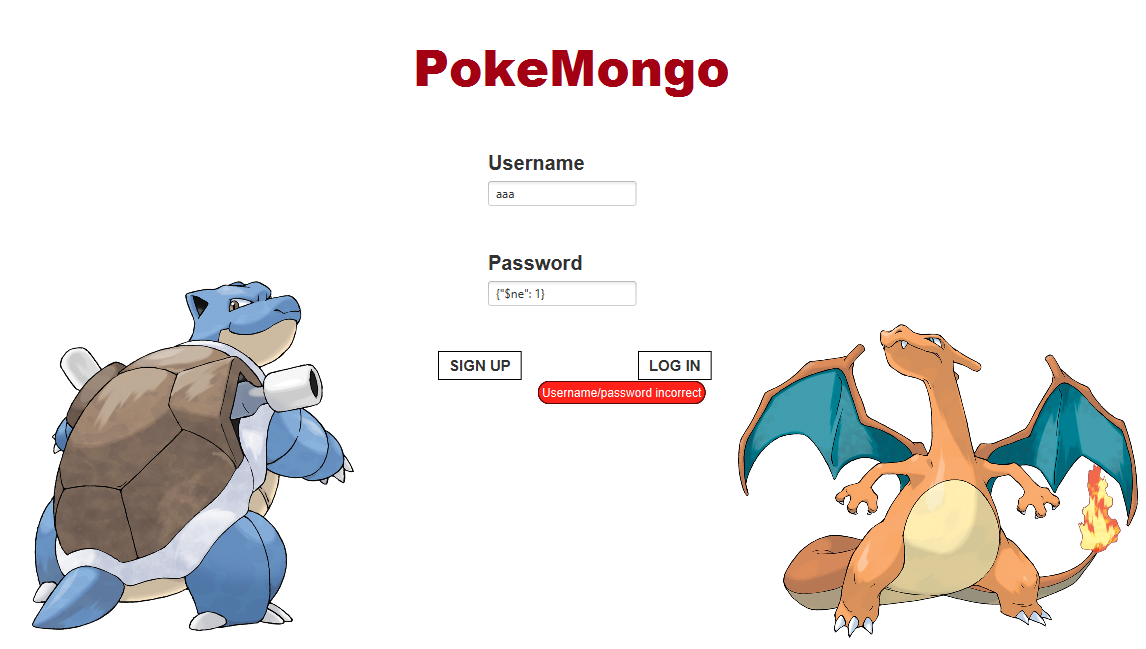
\includegraphics[width=\textwidth]{img/privacy_1.png}
\end{figure}
\begin{figure}[H]
	\centering
	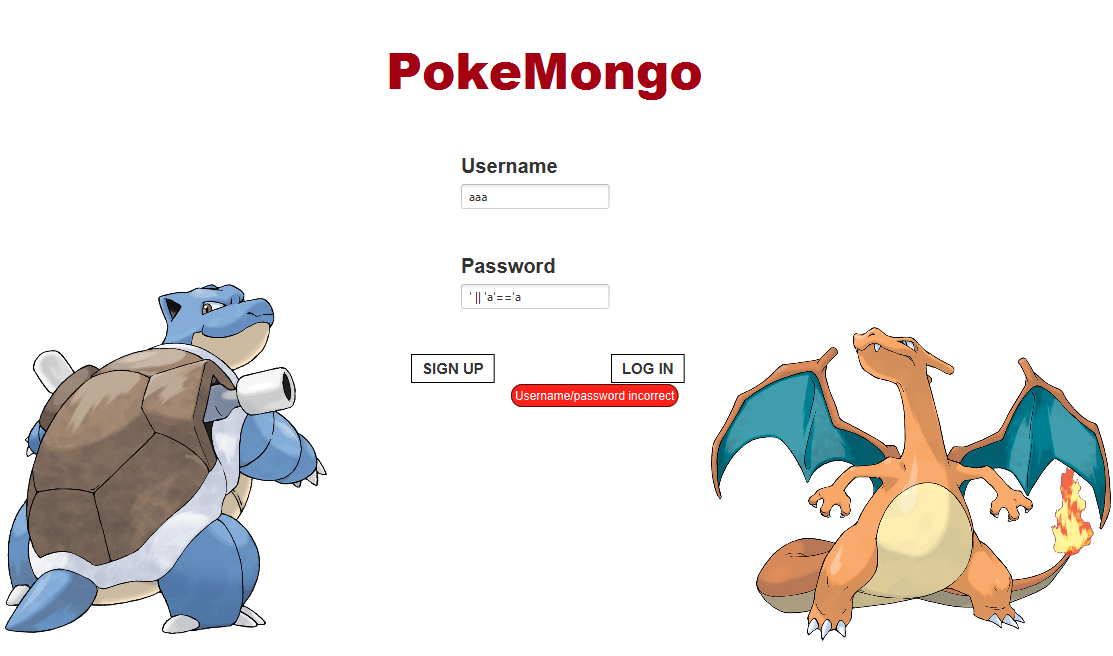
\includegraphics[width=\textwidth]{img/privacy_2.png}
\end{figure}


\begin{figure}[H]
	\centering
	\caption{Example 2: input validation on the signup form blocks code injection attempts (it would have removed all the collection)}
	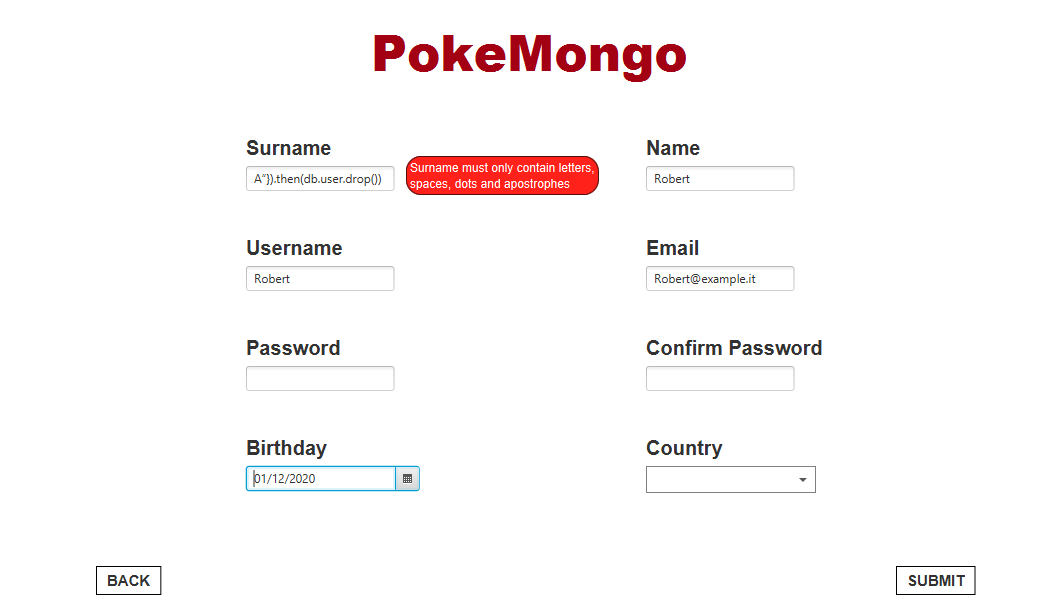
\includegraphics[width=\textwidth]{img/privacy_3.png}
\end{figure}


\subsection{Unit Test}
While writing the implementation of the various Classes of the project, Unit Tests were written in order to check if the modules were working properly. The main types of test written are the following:
\begin{itemize}
	\item \textbf{Singleton Check}: whenever a Singleton Pattern is implemented in a class there is a test that will check if two instance of the same class are the same. Here are some examples of these tests:
\begin{lstlisting}[language=Java]
//Cache
public void WHEN_getInstance_invoked_twice_THEN_same_ instance_returned(){
	PokeMongoImageCache pkic2 = PokeMongoImageCache.getInstance();
	Assertions.assertEquals(pkic, pkic2);
}
\end{lstlisting}
	\item \textbf{Exception Check}: in many parts of the code there will be tested if a particular input will generate or not an Exception (both cases are present). Here are some examples of these tests:
\begin{lstlisting}[language=Java]
//PokemonManagerOnMongoDb
public void WHEN_insert_invoked_with_non_Pokemon_
parameter_THEN_Exception_not_thrown(){
	Assertions.assertDoesNotThrow( ()->{
		PokemonManagerOnMongoDb pokemonManagerOnMongoDb = new PokemonManagerOnMongoDb();
		Object c = new Character('c');
		pokemonManagerOnMongoDb.insert(c);
	});
}
public void WHEN_update_invoked_with_non_Bson_parameter_
newvalue_THEN_Exception_not_thrown(){
	Assertions.assertDoesNotThrow( ()->{
		PokemonManagerOnMongoDb pokemonManagerOnMongoDb = new PokemonManagerOnMongoDb();
		Object c = new Character('c');
		pokemonManagerOnMongoDb.getWithFilter(c);
	});
}

//TeamManagerOnNeo4j NOTE THE "KISS" TEST
public void WHEN_getPokemons_invoked_with_non_
ArrayOfRecords_parameter_THEN_ClassCastException_thrown(){
	Assertions.assertThrows(ClassCastException.class, ()->{
		TeamManagerOnNeo4j teamManagerOnNeo4j = new TeamManagerOnNeo4j();
		
		Object c = new Character('c');
		ArrayList<Object> cList = new ArrayList<>();
		cList.add(c);
		ArrayList<Pokemon> arrayList = new ArrayList<Pokemon>();
		teamManagerOnNeo4j.getPokemons(arrayList, cList);
	});
}
\end{lstlisting}
	
	\item \textbf{Bad Input Check}: general check that a "bad input" (like an empty string, a NaN ...) in some particular classes will generate the predicted response. These tests are particularly performed in the \textbf{Form Validator}. Here are some examples of these tests:
\begin{lstlisting}[language=Java]
//FormValidatorPokeMongo
public void WHEN_isPersonNoun_invoked_with_empty_
string_THEN_false_returned(){
	Assertions.assertFalse(formValidatorPokeMongo.isPersonNoun(""));
}

public void WHEN_isValidEmail_invoked_with_empty_
string_THEN_false_returned(){
	Assertions.assertFalse(formValidatorPokeMongo.isValidEmail(""));
}

public void WHEN_isValidPassword_invoked_with_empty_
string_THEN_false_returned(){
	Assertions.assertFalse(formValidatorPokeMongo.isValidPassword(""));
}

\end{lstlisting} 
	\item \textbf{Security Check}: check of the goodness of the \textbf {Security} class in terms functionality with bad inputs, same output check with same input and so on. Here are some examples of these tests:
\begin{lstlisting}[language=Java]
//PasswordEncryptor
public void WHEN_encrypt_password_invoked_twice_
with_same_input_THEN_same_output_returned(){
	String out1 = PasswordEncryptor.encryptPassword("prova1");
	String out2 = PasswordEncryptor.encryptPassword("prova1");
	Assertions.assertEquals(out1, out2);
}

public void WHEN_encrypt_password_invoked_twice_
with_different_input_THEN_different_output_returned(){
	String out1 = PasswordEncryptor.encryptPassword("prova1");
	String out2 = PasswordEncryptor.encryptPassword("prova2");
	Assertions.assertNotEquals(out1, out2);
}

public void WHEN_encrypt_password_invoked_with_empty_
string_THEN_non_empty_output_returned(){
	String out = PasswordEncryptor.encryptPassword("");
	Assertions.assertNotEquals(out, "");
}
\end{lstlisting}
\end{itemize}
\subsection{Robustness}
In this paragraph we will analyse how much the application is (not) fault-tolerant with respect to \textbf{Users}’ wrong or mischievous behaviours, database inconsistencies and/or breakdown of one or more component of the application.

\subsubsection{Wrong inputs and mischievous behaviour}
As well as presented in the paragraph 5.1.3, a validator mechanism protects the application from any kind of wrong input, not only for what it concern data types (String input on a integer field), but also values.

\begin{figure}[H]
	\centering
	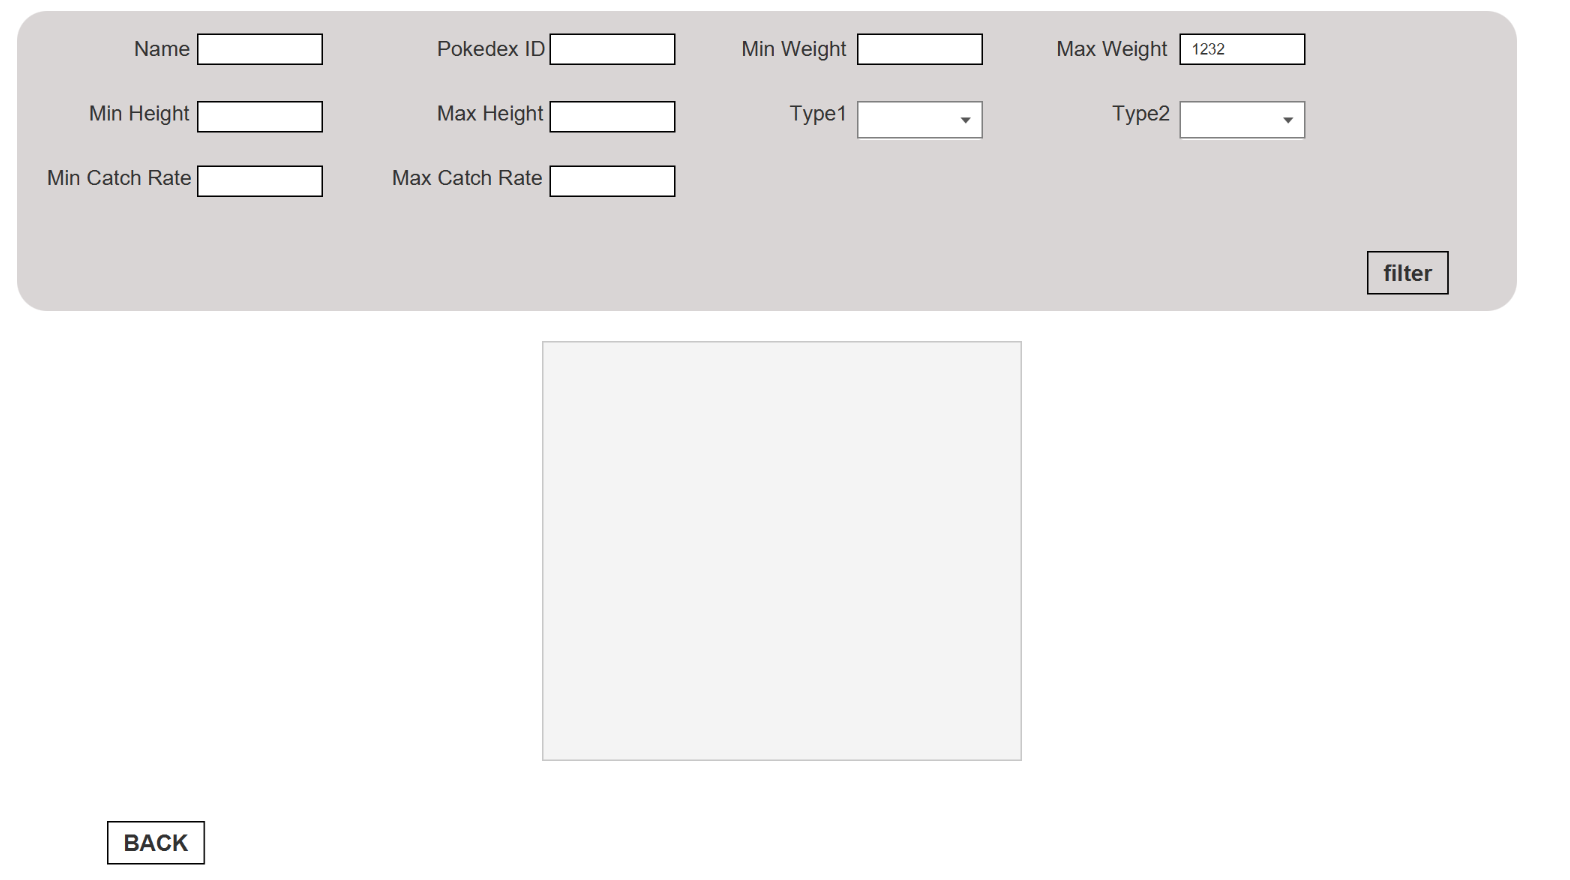
\includegraphics[width=\textwidth]{img/wrong_input.png}
\end{figure}

In the example reported, taken from the \textit{Pokédex} page, is not possible to input digits on alphabetical fields (like \textit{Name}), nor to insert letters in numerical fields(like \textit{Min Weight}). Moreover, no numerical field accept negative values (see \textit{Max Weight} in the previous picture), and since special characters are not allowed, there is no way to inject code.\\
The same features have been implemented in each alphabetical/numerical field; those examples are not here reported.\\
On the contrary, due to the fact that the remote connection to the database can generate some latency, the application is not robust w.r.t. quick and repetitive requests to the database. Indeed, submitting many requests in a short window of time increases the risk of an out-of-order arrival at the database side: in this way some strange but limited behaviour can appear.

\subsubsection{Database Inconsistencies}
By code, when a \textbf{User} is added/removed, the control does not come back until the \textbf{User} itself had been removed: this means that, in nominative conditions, there is no chance to create a \textbf{User} in a db and not to add it to the other database too.\\
Anyway, in case of inconsistencies due to possible errors/breakdowns, the application continues to run but it will fail often.\\
For example, if a \textbf{User} is inserted into MongoDB, but for any reason he/she is not added to Neo4J too, the \textbf{User} will continue to exist but he/she will not be able to build up a \textbf{Team}, nor to insert \textbf{Posts} and so on. The correct working of the application is crucially dependent on the correct behaviour of the databases.

\subsubsection{External Faults}
As discussed in the previous chapter, if the database fails the application is no more able to work correctly. Anyway, thanks to the log file, it will be extremely simple determining what went wrong.\\
Generalizing this discussion, the application is dependent on the following modules, for each of them we report the corresponding fail robustness of the system.
\begin{itemize}
	\item \textbf{Document Db} and \textbf{Graph Db} as discussed before are vital for the application
	\item A \textbf{Caching System} speeds up image loading (par. 4.3.2). If it fails, the application will still be available and capable of loading them but the \textbf{latency will be higher}
    \item The \textbf{Internet connection} is required also for the downloading of the Pokémon images (before caching). Let us suppose that we are no more able to connect ourselves to Internet but to have a backup connection through the databases: in this case the application will still work correctly, but non-cached images will not be displayed.
	\item A \textbf{configuration file} divides the parameter data from the applicative one, and modularizes the code. If this file goes lost or corrupted, a \textbf{default-values} collection inside ConfigDataHandler will ensure a sub-optimal but correct behavior of the application.
	\item The \textbf{Logger} has only event-recording purposes, in order to restore quickly possible faults. As specified in the paragraph 4.3.4 this tool is handled by a parallel thread, if it fails no consequences will be reflected into the application
	\item As discussed in the paragraph 3.6, admins’ analytic queries are handled by an \textbf{external client} that also strictly requires the correct working of the databases. 
	If this external client fails, analytic data will be no more updated, which means that a\textbf{dmins will visualize always the same data}; this event has no other impact on the application.  
	\item The \textbf{Password Encryptor} is involved to ensure the privacy of users’ sensible data. If, for any reason, this module stops working, there will be access problems for any user that will try to login. No issue will be experimented by users already logged.
\end{itemize}
